% !TEX root = morphkasten.tex

\section{Fahrbahnerkennung}


%##############
\subsection{Sensor}

\begin{figure} [hbp]
	\centering
	\begin{subfigure}[b]{0.4\textwidth}
		\includegraphics[width=\textwidth]{fig/Linienerkennung_1.png}
		\caption{1.Situation: Sensoren über der Linie}
	\end{subfigure}
	\hfill
	\begin{subfigure}[b]{0.36\textwidth}
		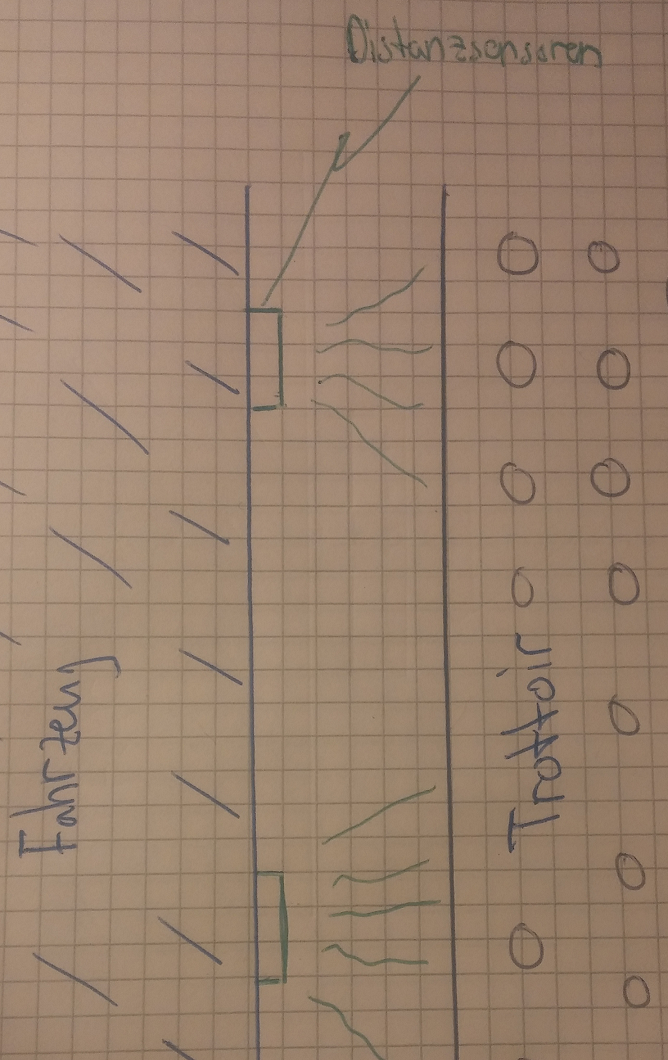
\includegraphics[width=\textwidth]{fig/Trottoirerkennung_1.png}
		\caption{2. Situation: Sensoren für die Abstandserkennung}
\end{subfigure}
	\caption{Mögliche Spurerkennung mit Distanzsensoren}\label{fig:animals}
\end{figure}



\begin{table}[h]
\begin{tabular}{p{0.5\textwidth} | p{0.5\textwidth}}


 \textbf{Vorteile} & \textbf{Nachteile} \\ \hline
	 
\begin{itemize}
\item Gut zu testen (Funktionsmuster)
\item Gute Präzision wird erwartet
\end{itemize}

 
 &
 
\begin{itemize}
\item Braucht externe Hardware und Verkabelung
\item Funktionsmuster zwingend notwendig
\end{itemize}

\end{tabular}
\end{table}

\begin{table}[h]
\begin{tabular}{p{0.5\textwidth}p{0.5\textwidth}}

 \textbf{Risiken} & \\ \hline
	 
\begin{itemize}
\item Die Linie lässt sich nicht Erkennen (ohne Konflikte mit der Anforderungsliste)
\item Das Trottoir ist zu wenig hoch damit es sich erkennen lässt
\end{itemize}
&
\begin{itemize}
\item Die Steuerung aufgrund der Linienerkennung ist nicht praktikabel
\end{itemize}

 
\end{tabular}
\end{table}

\pagebreak


%##############
\subsection{Bilderkennung}
Grafik

\begin{table}[h]
\begin{tabular}{p{0.5\textwidth} | p{0.5\textwidth}}


 \textbf{Vorteile} & \textbf{Nachteile} \\ \hline
	 
\begin{itemize}
\item Vorteil 1
\item Vorteil 2
\item Vorteil 3
\item ...
\end{itemize}

 
 &
 
\begin{itemize}
\item Nachteil 1
\item Nachteil 2
\item Nachteil 3
\item ...
\end{itemize}

\end{tabular}
\end{table}

\begin{table}[h]
\begin{tabular}{p{0.5\textwidth}p{0.5\textwidth}}


 \textbf{Risiken} & \\ \hline
	 
\begin{itemize}
\item Risiko 1
\item Risiko 2
\end{itemize}
&
\begin{itemize}
\item Risiko 3
\item ...
\end{itemize}

 
\end{tabular}
\end{table}

\pagebreak